\documentclass{osa-article}
\usepackage{amsmath}
\usepackage{cite}
\usepackage{float}
\usepackage{textgreek}
\journal{oe}
%% \articletype{Research Article}


\newtheorem{theorem}{Theorem}
\newtheorem{lemma}{Lemma}

\begin{document}

\title{Flexible Dual-soliton Manipulation for Coherent Anti-stokes Raman Scattering Spectroscopy}

\author{Tao Wu,\authormark{1} Kun Chen,\authormark{1,2} Huijie Zhao,\authormark{1} Weipeng Zhang,\authormark{1} Yan Li\authormark{1} and Haoyun Wei\authormark{1,*}}

\address{\authormark{1}State Key Lab of Precision Measurement Technology and Instrument, Department of Precision Instrument, Tsinghua University, Beijing 100084, China\\
\authormark{2}Department of Chemistry, University of California, Berkeley, CA 74920, USA} 

\email{\authormark{*}luckiwei@mail.tsinghua.edu.cn}


\begin{abstract}
Though dual soliton is used as the Stokes source in coherent anti-Stokes Raman scattering (CARS) experiments, the mechanism behind it is still not fully investigated. In this paper, dual-soliton pulses generation with a highly birefringent photonic crystal fiber (PCF) is numerically explored and experimentally verified. The simulated pulse exhibits various characteristics in the temporal and spectral domains with respect to the input linear polarization angle, and can be classified into four regions based on distances in the temporal and spectral domain of the soliton pair. By tuning input power and polarization angle, a soliton pair with desirable spectral coverage and temporal delay for CARS applications can be flexibly generated before the two solitons overlap in time domain. The simulated results are then experimentally validated by comparing their temporal and spectral characteristics. In addition, the benefit of using dual-soliton sources, such as Stokes beam, in CARS experiments is also demonstrated. The results and methods presented in this work can improve CARS spectroscopy and microscopy techniques, and may also be beneficial to other dual-wavelength source applications.
\end{abstract}


\section{Introduction}

Ultrafast fiber pulsed lasers, with their remarkable performance and competitive cost, are broadly used in coherent Raman scattering(CRS) microscopy research\cite{andresen_tunable_2006, andresen_stimulated_2011, Gottschall.2015, Krafft.2016}. However, with the advancement of CRS techniques and applications, researchers are seeking superior performance light sources. For example, in biology, detecting the fingerprint region, where most Raman peaks are located, needs Stokes light that is tunable from 1.1 \textmu m to 1.3 \textmu m for Yb-doped pump lasers\cite{Gottschall.2015}. To acquire video-rate hyperspectral Raman images, the stimulated pulses are expected to have broad spectral coverage. In physics, larger single-pulse energy is advantageous to exciting more energy levels. For general users, the light source is expected to be more robust, stable, space- and cost-efficient. Fiber lasers are insufficient as a light source, since its output power and spectrum are significantly limited by the gain medium and resonant cavity. In combination with fiber lasers, the soliton self-frequency shift (SSFS), which enables continuous wavelength tuning of a soliton via intra-pulse Raman scattering, provides a promising route to fulfilling many of the above expectations, and has proved to be efficient in several applications\cite{Paulsen2003,yuan_red-shifted_2015,Li.2017}. Among the nonlinear media used in demonstrating SSFS, photonic crystal fibers are becoming more and more popular in the past decades. By using silica glass-based PCFs, the wavelength tuning of soliton sources from 0.85 \textmu m to 1.05 \textmu m\cite{Su2013}, 1.03 \textmu m to 1.4 \textmu m\cite{Andresen.2007} and 1.580 \textmu m to 2.130 \textmu m\cite{wang.2011} have been reported. Recently, dual-soliton generated in highly birefringent PCF brought new research opportunities. The generated dual-soliton pulses sweep through temporal and spectral intervals, from incidence to several picoseconds or tens of nanometers as the input power and polarization changes. This flexibility leads to the realization of a background-free\cite{chen_dual-soliton_2016} and broadband\cite{chen_cascaded_2016} CARS technique under different dual-soliton configurations. For dual-comb CARS systems\cite{ideguchi_coherent_2013, mohler_dual-comb_2017}, using dual-soliton configuration is equivalent to doubling the repetition frequency and, therefore, improves the duty cycle of the measurement. Compared with solitons from single mode PCFs \cite{klarskov_supercontinuum_2011,arteaga-sierra_supercontinuum_2014,Qiu.2014}, which are discussed in many research studies, dual-soliton generation involves an extra degree of freedom for the input polarization angle (the angle between input polarization and fast axis of PCF)and several nonlinear effects, including cross-phase modulation and polarization-mode dispersion. Therefore, it is worth exploring its evolution in a more systematic and comprehensive manner to evaluate and predict its characteristics and provide guidance on CARS spectroscopy and other potential optical applications. 

In this paper, we numerically and experimentally investigate the cross-axis interaction effect in highly birefringent PCFs with respect to input power and polarization angle. The physical model includes all major nonlinear effects and the simulation is conducted efficiently, and benefits from graphic card computing acceleration and advanced numerical method. We found that with our experiment configuration, dual soliton can be generated in the spectral range of around 1.150 \textmu m to 1.350 \textmu m, and their relative temporal and spectral relationships can be tuned flexibly and easily. For other kinds of highly birefringent PCFs, we believe the evolution characteristic of the dual soliton remains so that desirable soliton pairs can also be found. In the last section of this paper, we present results from our dual-soliton CARS investigation to demonstrate its capability to facilitate CARS microspectroscopic application. 
\section{Methods}

For investigating the properties of dual-soliton generation in the PCF, a well-known vector generalized nonlinear Schrodinger equation (VGNLSE)\cite{husakou_supercontinuum_2001,agrawal_nonlinear_2013} is adopted in this simulation. This equation uses the complex envelope of the electric field and assumes that the time origin moves with light pulses, which greatly simplifies the calculation. Most of the nonlinear effects in fiber are taken into consideration, including self-phase modulation(SPM), cross-phase modulation(XPM), intra-Raman scattering, and higher-order dispersion and self-steeping so that the equation is applicable for cases where pulses are shorter than 100 fs\cite{agrawal_nonlinear_2013}. As the fiber is highly birefringent, the refractive index difference is also considered. However, the effect of four-wave mixing(FWM) is ignored, as the phase-matching condition is hardly satisfied in highly birefringent fibers. Compared to our previous study\cite{chen_dual-soliton_2016}, equations in this paper are improved and yield more accurate results.  

\begin{equation}
\begin{split}
\frac{\partial u}{\partial z} - & i\beta u + \delta \frac{\partial u}{\partial t}-\sum_{k=2-6}\frac{i^{k+1}}{k!}\beta_k\frac{\partial^k u}{\partial t^k} =\\
 & i\gamma\left(1+\frac{i}{\omega_0}\frac{\partial}{\partial t}\right)\left(|u|^2+\frac{2}{3}|v|^2+u\int_0^\infty{R(t')|u(t-t')|^2dt'} \right)
\label{eq1}
\end{split}
\end{equation}


\begin{equation}
\begin{split}
\frac{\partial v}{\partial z} + & i\beta v - \delta \frac{\partial v}{\partial t}-\sum_{k=2-6}\frac{i^{k+1}}{k!}\beta_k\frac{\partial^k v}{\partial t^k} =\\
 & i\gamma\left(1+\frac{i}{\omega_0}\frac{\partial}{\partial t}\right)\left(|v|^2+\frac{2}{3}|u|^2+v\int_0^\infty{R(t')|v(t-t')|^2dt'} \right)
\label{eq2}
\end{split}
\end{equation}

In Eq.\ref{eq1} and Eq.\ref{eq2}, u and v are the envelopes of the optical pulses in the two principle axes. The linear terms are on the left side and nonlinear ones are on the right. $\beta=\pi/L_b$ is the wavenumber difference between the two modes, and $L_b$ is the beat length of the birefringent fiber. $\delta=\beta \lambda/(2\pi c)$ is the inverse group velocity difference. $\beta_k$ is the k-th-order dispersion coefficient. $\gamma$ is the nonlinear coefficient. $\omega_0$ is the center frequency of the input pulse. $R(t)$ is the Raman response of the fiber material. Here, a model including thirteen vibration modes is used\cite{Hollenbeck2002}. This model is closer to the experimental data but does not increase computing complexity.

\begin{equation}
    R(t)=f_r\sum_{i=1-13}\frac{A_i '}{\omega_{v,i}}\exp(-\gamma_i t)\exp(-\Gamma_i^2t^2/4)\sin(\omega_{v,i}t)\theta(t)
    \label{eq3}
\end{equation}

In Eq.\ref{eq3}, $f_r$ is set as $5.8\times 10^{10}$ such that the height of the first peak of $R(t)$ matches those in the other simulations\cite{agrawal_nonlinear_2013}. All other parameters are defined in Ref.\cite{Hollenbeck2002}.

All the parameters used in our simulations are set to match the experimental conditions in the next section. Specifically, a commercial highly birefringent PCF (NKT Photonics SC-5.0-1040-PM) is used as the nonlinear medium. The related parameters are determined as follows: $\beta_2=-2.93\times 10^{-27} s^2m^{-1}$, $\beta_3=7.17\times 10^{-39} s^3m^{-1}$, $\beta_4=-1.19\times 10^{-55} s^4m^{-1}$, $\beta_5=4.14\times 10^{-70} s^5m^{-1}$, $\beta_6=9.93\times 10^{-85} s^6m^{-1}$, $\gamma=0.011 W^{-1}m^{-1}$, $\lambda=1060 nm$. $L_b=6.3 mm$ and PCF length is $ L=1.93m$. The input pulse is assumed to be Gaussian-shaped with a Fourier transform-limited full width at half maximum(FWHM) of 65 fs, according to the autocorrelator. Then, the pulse is stretched by second-order dispersion of 3000 fs\textsuperscript{2} to compensate for the chirps introduced before entering the PCF. In addition, the input power is examined to ensure it is in a suitable range that is strong enough for cross-axes effects but will not generate higher-order solitons or supercontinuum. It is worth noting that the high-order dispersion parameters are re-calculated from the dispersion curve provided by NKT and may be different from those in previous research studies\cite{chen_dual-soliton_2016}.

The equation is numerically solved by the fourth-order Runge--Kutta in the interactive picture (RK4IP)\cite{Hult2007} method. The program is written in CUDA C/C++ with Visual Studio. As the algorithm is implemented on a graphic card, the simulation speed is relatively fast even with a middle-range GPU(GTX 1050Ti, NVIDIA). All the step parameters are tested for convergence while keeping the amount of calculation as small as possible. The source code is uploaded to Github for verification and simulation of other nonlinear phenomena.


\section{Simulation results and discussion}

\begin{figure}[htbp]
    \centering%
    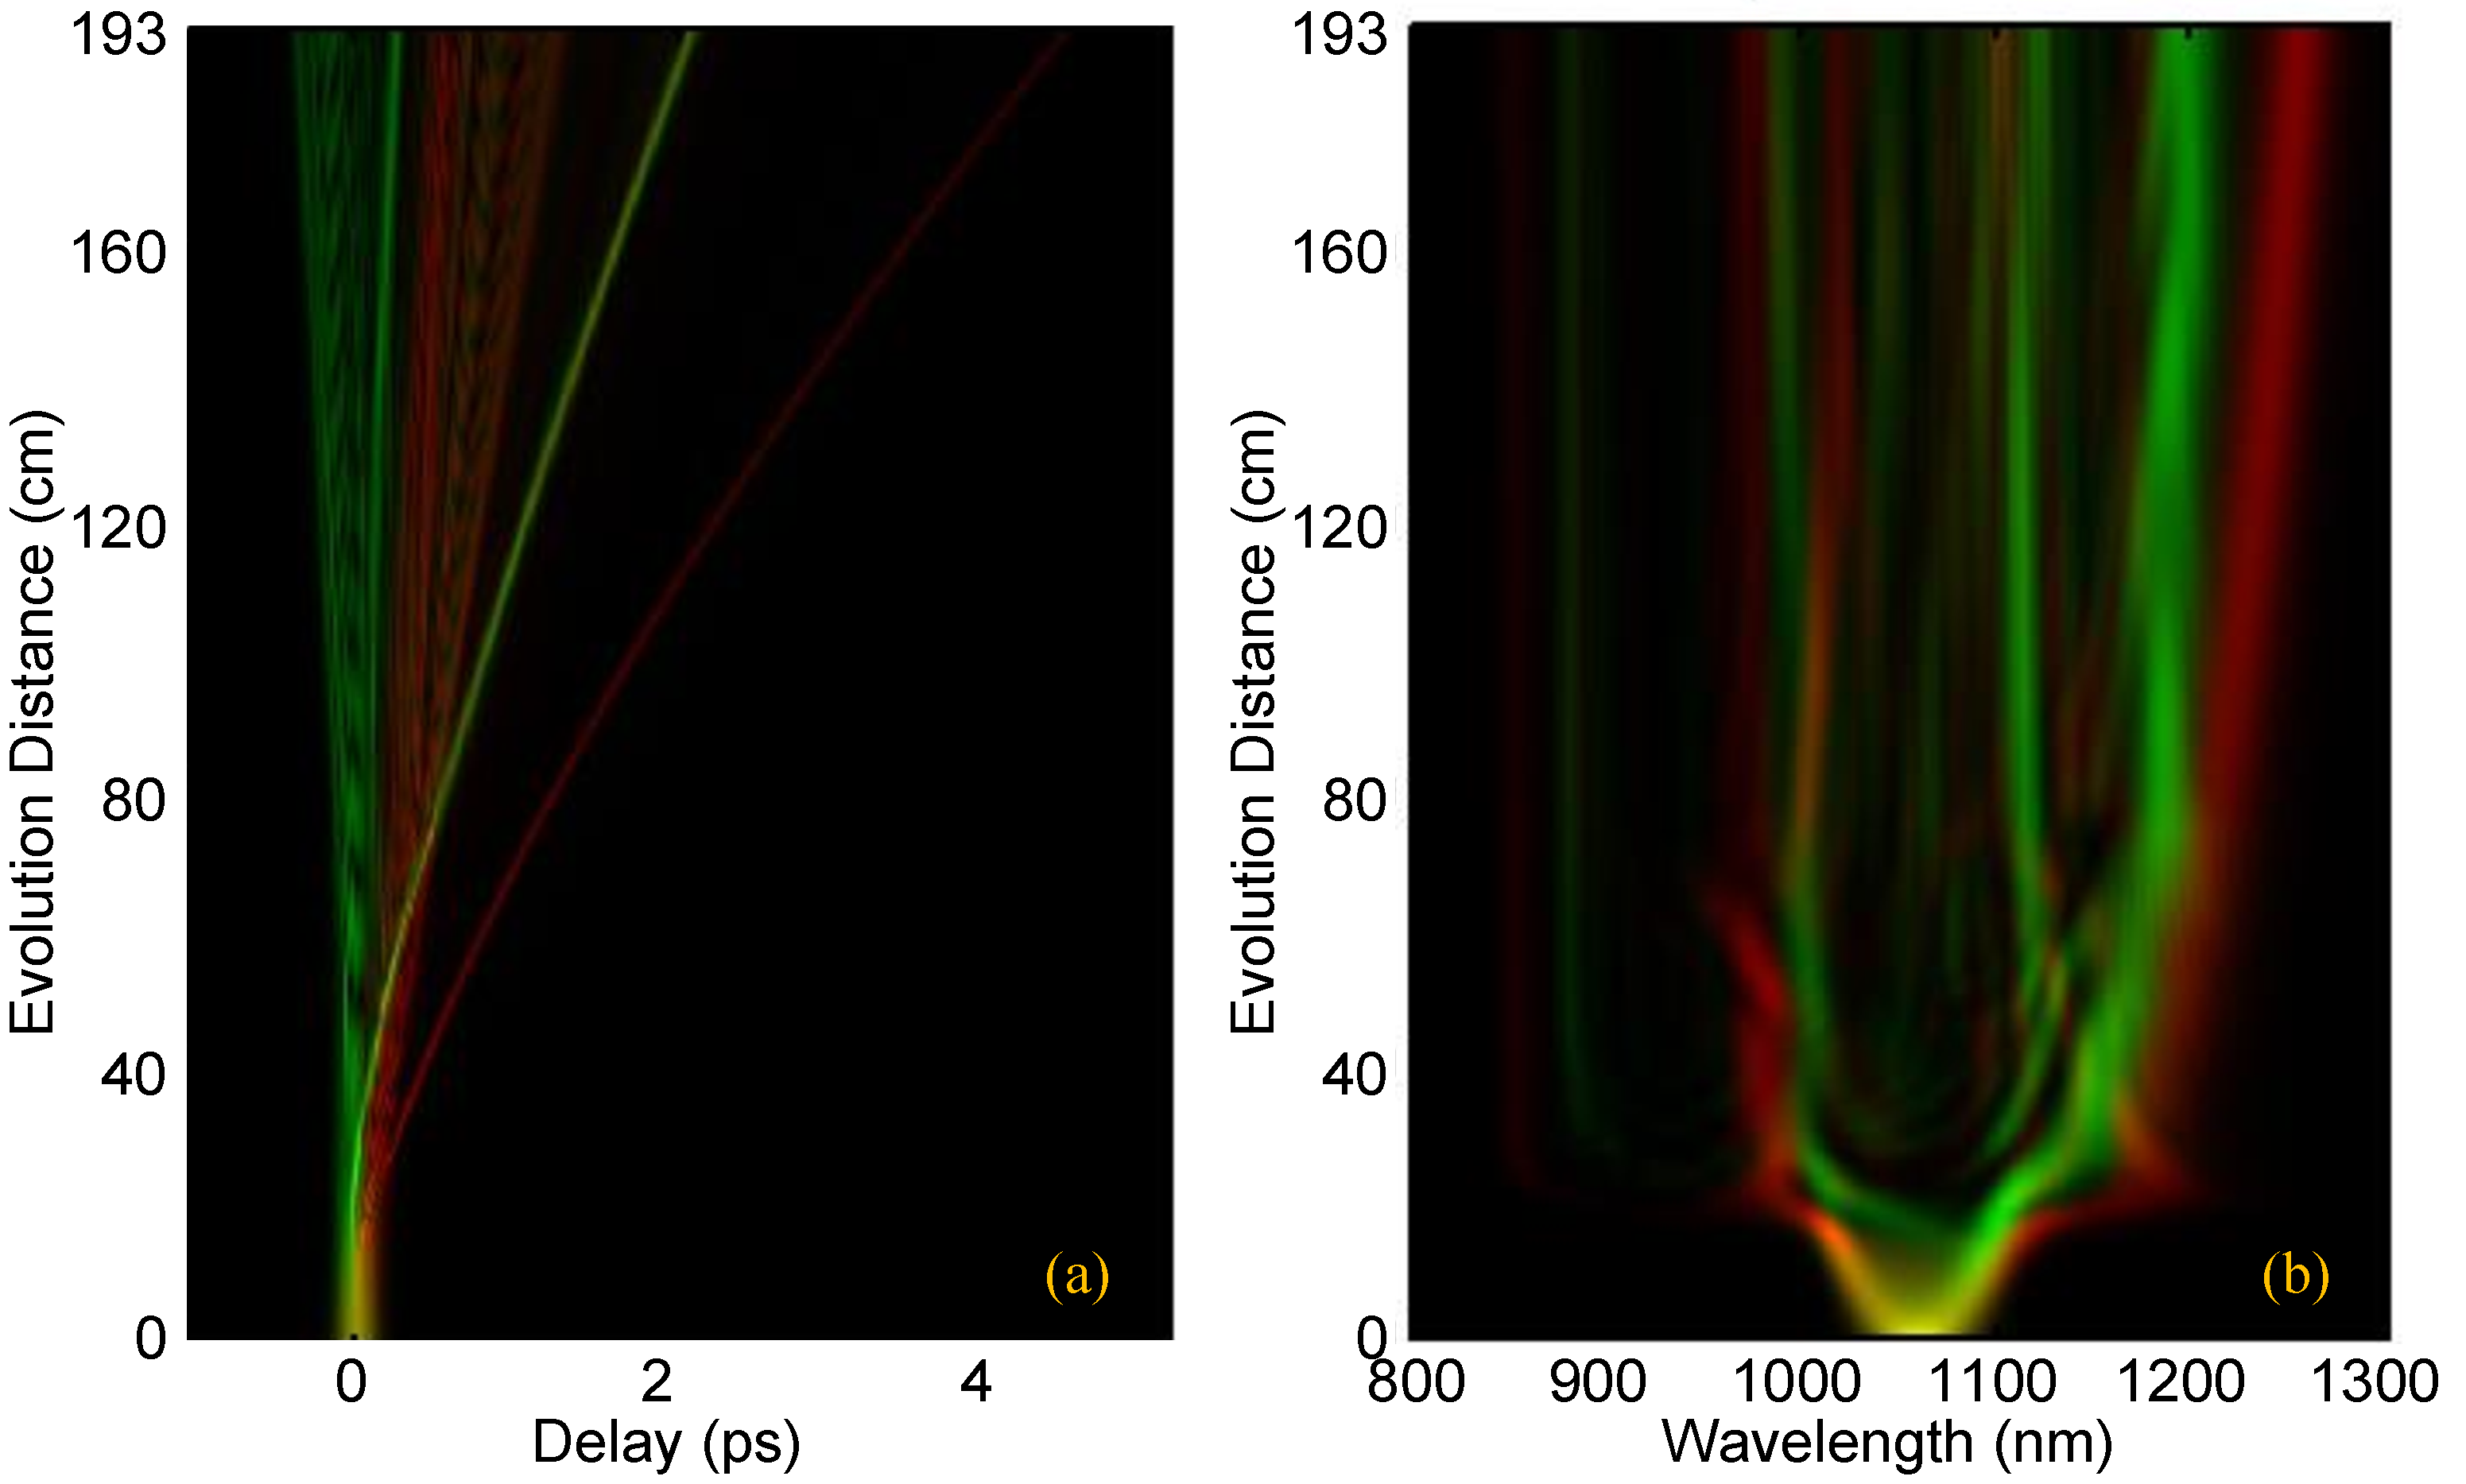
\includegraphics[width=300pt]{fig_propagation.pdf}
    \caption{Temporal (a) and spectral (b) evolution along evolution distance. Red color for fast axis and green for slow axis.}
    \label{fig_propagation}\vspace*{-6pt}
\end{figure}
 
Fig.\ref{fig_propagation} shows the temporal and spectral evolution of a pulse in the highly birefringent PCF, the input power is around 80 mW and input polarization angle is 30 degrees. SSFS occurs after propagating a short distance along both the axes. In the temporal domain (a), the dominant soliton in each axis is nearly transform-limited. However, the soliton in the slow axis looks a bit yellow in color, indicating that a weak soliton in the fast axis is locked to it. Clearly, the cross-axis effect plays a key role here. In spectral domain (b), both solitons move toward higher wavelengths as the distance increases, like many other simulations\cite{dudley_supercontinuum_2006}. The spectrum of the slow soliton is distorted as a result of the weak soliton in the fast axis. Regardless, it is easy to find that both the center wavelength and the delay difference of the two dominant solitons increase with propagation along the highly birefringent PCF.

\begin{figure}[htbp]
\centering%
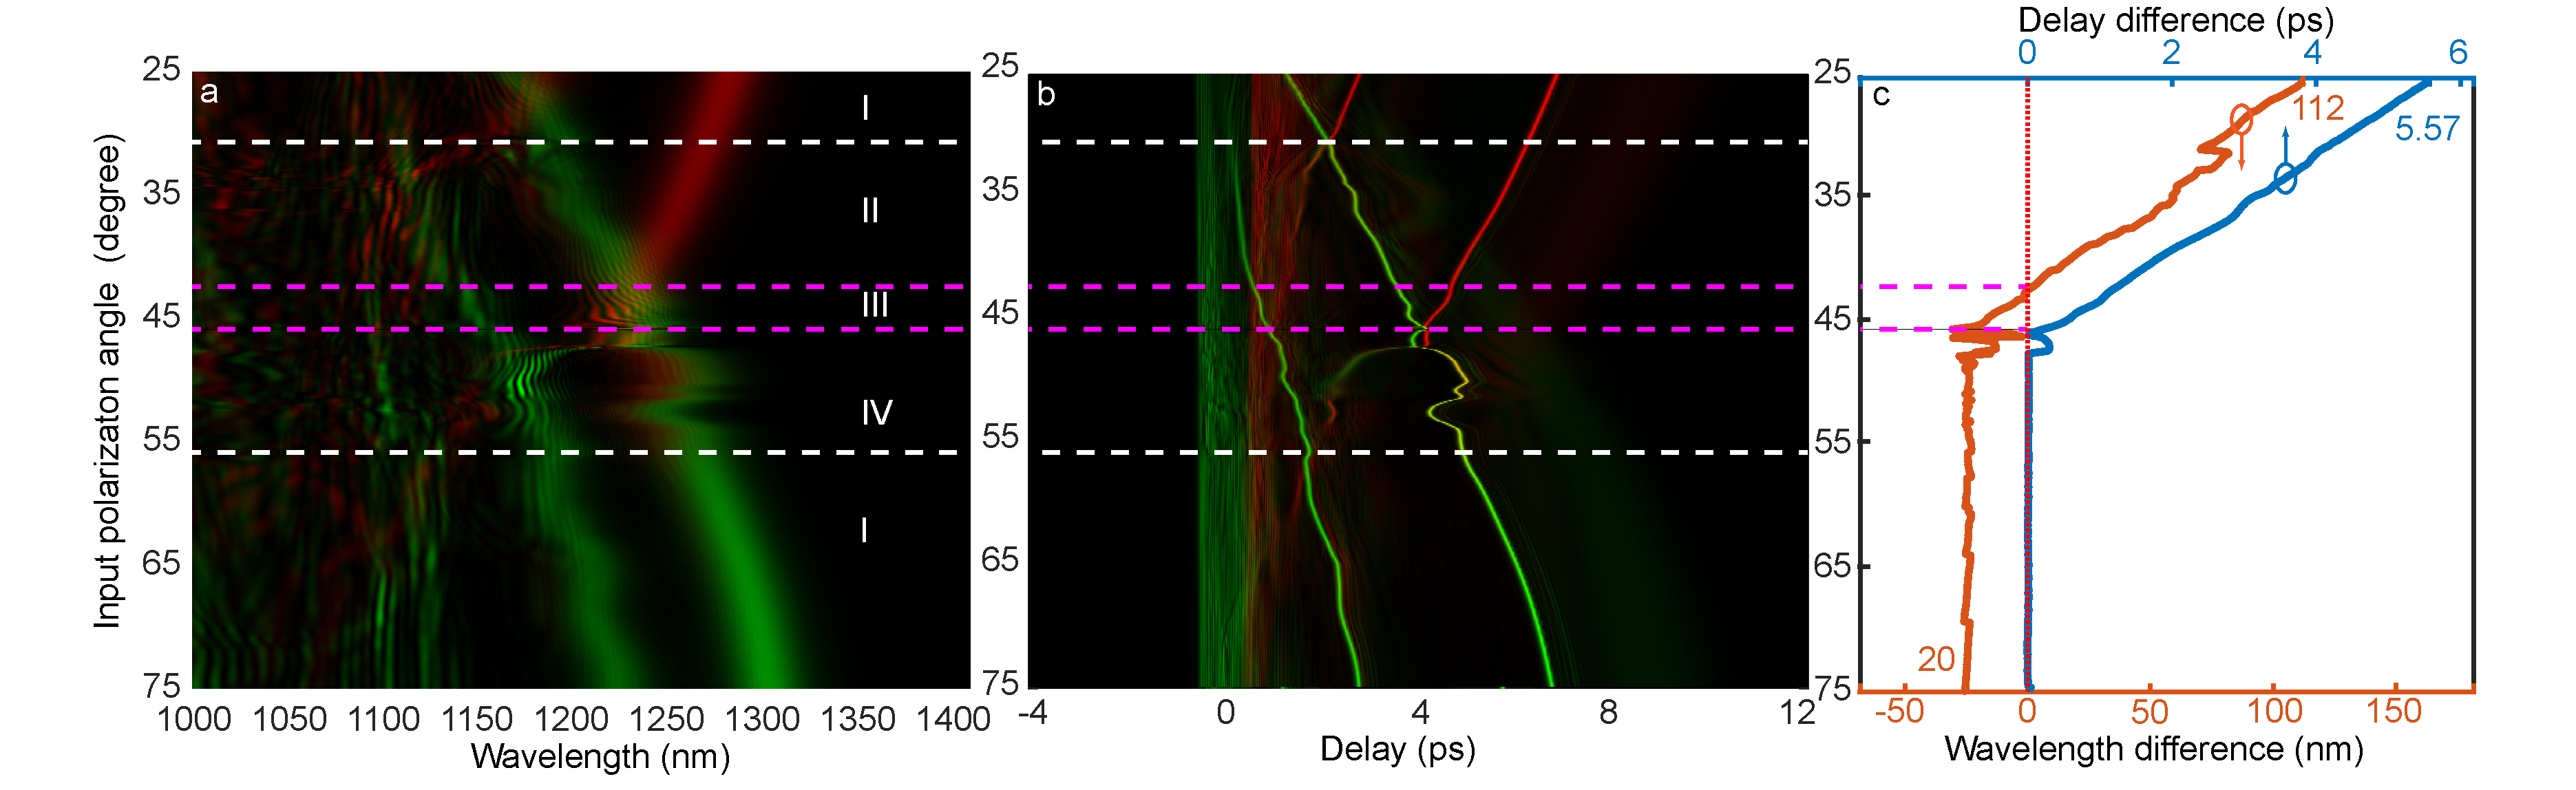
\includegraphics[width=\textwidth]{fig_sim.pdf}
\caption{Output evolution at different input polarization angles. (a) Output spectra against input angle. The red and green value in each pixel is the intensity in the fast and slow axes, respectively. (b) Output pulses in temporal domain. (c) Wavelength (orange) and delay (blue) difference at different input polarization angles.}
\label{fig_C}\vspace*{-6pt}
\end{figure}

Fig.\ref{fig_C} shows a typical numerical result in the spectral domain (a) and the temporal domain (b) with different input polarization angles when the input power is set to 80 mW. The whole graph is not symmetric to 45 degrees due to the high refractive index differences in different axes. It is straightforward to find that lower-order solitons are generated in both the fast axis (shown in red) and the slow axis (shown in green). However, when the input linear polarization angle is out of the range of around 30 degrees to 55 degree, marked as region I in Fig.\ref{fig_C}, only solitons generated in one axis dominate the output. As the cross-axis effect is negligible, changing polarization angle is equivalent to changing input power. The soliton tuning treading is quite straightforward. When the input angle is between 30 and 55 degrees, the cross-axis effect plays a key role in propagation, and this region can be further classified into three regions, namely, regions II, III, and IV, according to their tuning characteristics. In region II, although it seems that the two dominant solitons are not overlapping in both the domains, we observe on Fig.\ref{fig_propagation} that a weak soliton in the fast axis is found to be locked to the dominant soliton in the slow axis. As the input polarization angle increases from around 30 degrees, the dominant solitons in both the axes come closer in both the spectral and temporal domains, while the one in the fast axis has a larger center wavelength and relative delay, which is quite understandable as the input power of the two axes get closer. The changes in both the domains are almost linear, as shown in Fig.\ref{fig_C}(c), until the solitons are overlapped in the spectral domain. Then, the delay difference continues to decrease linearly until zero. This region, between the spectral and temporal crossing points, is named as region III. After the solitons collapse in the temporal domain, they appear to be locked together. Their relative delay and center wavelength difference remains almost constant. However, their center wavelength and relative delay are sensitive to the input polarization angle until the input energy is not sufficient for the nonlinear cross-axis effects. This region is named as region IV, as shown in Fig.\ref{fig_C}, and is around 45 to 55 degrees. In this region, it is hard to get a desirable center wavelength and the output is too unstable for most applications. Then, it circulates back to region I, where intra-axis effects dominate.


\begin{figure}[htbp]
\centering%
\includegraphics[width=320pt]{fig_tuning.pdf}
\caption{Change of tuning characteristics at different average input powers. (a) Temporal(blue) and spectral(red) crossing points at different input powers (b) Center wavelength (blue) with temporal crossing and relative delay with spectral crossing at different input powers. (c) Center wavelength(blue) and relative delay(red) with input polarization angle is 35 degrees at different input powers }
\label{fig_tuning}\vspace*{-6pt}
\end{figure}

For dual-soliton CARS applications\cite{chen_dual-soliton_2016,chen_quantitative_2016}, the tuning characteristics of the solitons are more important. Therefore, changing trends of center wavelength and relative delay in region II and region III with respect to different input powers and polarization angles need further exploration.  

In order to subtract the nonresonant background in CARS detection, the two pulses' center wavelengths should be close but not exactly the same\cite{rocha-mendoza_differential_2009}. As shown in Fig.\ref{fig_tuning}(b), for different average input powers, when collapsed in the spectral domain, the relative delay is always around 1 ps, while the center wavelength increases as input power increases. This indicates that only a little adjustment in polarization angle, around 42 degrees, is needed for generating a soliton-pair with a 3-nm center wavelength difference. Meanwhile, the relative delay allows clear distinguishing between CARS signals of two solitons. Also, from Fig.\ref{fig_tuning}(b), it should be quite easy to get soliton with center wavelength from 1.19 \textmu m to 1.3 \textmu m. If a Yb-doped fiber laser is used as the pump pulse and the generated dual-soliton pulse is used as Stokes pulse, the covered Raman region is from 1030 cm\textsuperscript{-1} to 1741 cm\textsuperscript{-1}. If the spectral width of both the pulses, which is typically more than 10 nm, are taken into consideration, the detectable Raman region should cover more than 1200 cm\textsuperscript{-1}. However, in Fig.\ref{fig_tuning}(a), the two crossing points are getting quite close at high input powers, where higher-order solitons are generated. The shrinking region III indicates drastic change in the center wavelength and relative delay, making it quite hard to get desirable soliton pairs.

For CARS application, where broadband excitation is needed, it is also possible to find suitable soliton pairs in region II. Fig\ref{fig_tuning}(c) shows wavelength and relative delay change at different input powers. In this scenario, the relative delay is not the main concern as long as the delay is large enough to separate the signals. In region II, the center wavelength increases nearly linearly as input power increases, while the wavelength difference of two solitons changes with input polarization angle as revealed in Fig.\ref{fig_C}(c). Therefore, it should be easy to get solitons covering arbitrary Raman peaks in fingerprint region by adjusting the input power and polarization angle together. These flexibly manipulating features are attractive for CARS applications as they provide extra capacity to extend the detection of Raman spectral bandwidth or to focus pulse power on selected Raman peaks to achieve high sensitivity.

For region IV, the two solitons keep a center wavelength difference for about 20 nm. However, the pulses are locked up in temporal domain, strong inter-axis effects cause drastic changes in center wavelength as input polarization angle and power change. It is hard to get a desirable center wavelength and the poor stability is a drawback for continuous measurement. While their spectra are not fully overlapped, they are also not suitable for polarization sensitive CARS as well\cite{Hofer2017}. Even this region will never be used for nonlinear optics experiments, but at least it gives an intuitive demonstration of soliton locked-up case in a polarization sensitive waveguide.   

\section{Experiment}


\begin{figure}[htbp]
    \centering%
    \includegraphics[width=350pt]{fig_sys.pdf}
    \caption{Experiment Setup. HWP: half-wave plate, 1 and 2 are motorized, F: spectral filter, FM: flip mirror, GR: SF57 glass rod, DM: dichroic mirror, P: polarizer, OBJ: objective lens, PBS: polarized beam splitter, Spc: spectrometer, Det: detector, Acr: autocorrelator.}
    \label{fig_EC}\vspace*{-6pt}
\end{figure}


To validate the simulation results, an experiment was conducted to obtain the output spectra at different input polarization angles and different average powers. As shown in fig \ref{fig_EC}, the experimental setup is similar to our previous research\cite{chen_dual-soliton_2016}. In the experiment, a tailored mode-locked Yb-doped fiber laser with a chirped pulse amplifier is used as the light source. The output power is about 2 W and the repetition frequency is 100 MHz with center wavelength at 1.06 \textmu m when the minimum pulse width is reached. The minimum pulse width shown in an autocorrelator (APE PulseCheck) is 65 fs when the linear chirp is carefully compensated inside the laser. However, the sideband indicates the existence of higher-order dispersion. The input power is controlled by the combination of a half-wave plate and a polarization beam splitter (PBS). The input polarization angle is controlled by a second half-wave plate. Both the plates are controlled by a computer. The light is first coupled into a single–mode fiber which is spliced to the PCF for protection. The dispersion of the single-mode fiber broadened the light pulse just before it entered the PCF. The coupling efficiency is estimated to be around 30\% based on the ratio of output power and input power at low average input power. The length of the PCF is 1.93 m, which is the same as the value obtained from the simulation. Pulses generated from PCF are filtered by a long-pass filter (FEL1150) and delivered to a spectrometer (Ocean optics) or autocorrelator by coupling into single-mode fiber. A computer synchronizes the rotation of the second half-wave plate and acquisition from the spectrometer. The half-wave plate rotates from 0 to 90 degrees with a step size of 0.1 degrees and the spectrum is acquired and saved in each step.

\begin{figure}[htbp]
\centering%
\includegraphics[width=320pt]{fig_compare.jpg}
\caption{Comparison between simulation and experiment result. (a) Spectra from experiment, a 1150 nm long-pass filter is applied. (b) Spectra from simulation, input average power is set to 80 mW with zero dispersion. Artificial blurring is added to match the resolution of spectrometer used in experiment (c) Autocorrelator graph at 42 degrees from experiment (d) Simulated autocorrelator graph from simulation at 42 degrees.}
\label{fig_cmp}\vspace*{-6pt}
\end{figure}

The comparison of spectrum evolution against input polarization angle between simulation and experiment is shown in Fig. \ref{fig_cmp}. The simulation graph is the scalar addition of two axes where no polarization leakage is assumed to happen. Generally, the trends of spectrum evolution against input polarization angle are consistent. Region I to IV can be observed easily in the experiment. Typical patterns at 28 degrees and 50 degrees can be found in both the graphs. Besides, at the spectral crossing point, the autocorrelator waveforms (c) and (d) show an almost identical relative delay. The differences in the baseline and relative peak heights are simply the result of the instrumental response function of the autocorrelator. Although the two graphs are not exactly the same, it is feasible to analyze the evolution with simulation results. The differences between experiment and simulation come from many sources. For the input pulse, its waveform and power change with propagation in the single mode fiber before PCF. The intrinsic random noise can also cause significant variation in output\cite{dudley_supercontinuum_2006}. For PCF itself, nonlinear coefficient and dispersion difference in two axes are not taken into consideration because of a lack of data. Outside the PCF, the spectrum may get distorted as a combined effect of polarization leakage and uneven response of the spectrometer.


\begin{figure}[htbp]
    \centering%
    \includegraphics[width=\textwidth]{fig_cars.pdf}
    \caption{Original and processed Raman result of different samples. (a) Dual-soliton detection of fish oil: 1)original spectra signal, 2)signal from each soliton, 3)retrieved background-free Raman spectrum. (b) Cascaded detection of Polystyrene (PS) and polyethylene glycol terephthalate (PET): 1)original spectra, 2) signal from each soliton, 3)combined Raman spectrum. The spectrometer could be replaced by a highspeed detector.}
    \label{fig_CARS}\vspace*{-6pt}
\end{figure}

To demonstrate its advantages in CARS application, spectral focusing CARS technique with mechanical delay line is implemented as shown in Fig.\ref{fig_EC}. From Fig.\ref{fig_CARS}(a-1) and (b-1), the effect of dual-soliton excitation can be clearly found. For background-free detection(a), the two solitons are adjusted to have 3 nm and 1.3 ps differences in spectral and temporal domains, respectively. The CARS signal from each soliton is separated as shown in Fig.\ref{fig_CARS}(a-1) and is summed up independently along wavelength(a-2). Then, after the application of a certain algorithm \cite{chen_dual-soliton_2016}, the original Raman spectrum can be retrieved with non-resonant background significantly suppressed. For broadband detection(b), the two solitons are optimally controlled to focus on selected Raman peaks of PS beads and PET. After a sum up in wavelength (b-2) and phase retrieval, high signal-to-noise CARS signal with broadband coverage is achieved, as shown in Fig.\ref{fig_CARS}(b-3). Both the position and intensity of characteristic peaks in the demonstration are in accordance with those in spontaneous Raman spectra.  


\section{Conclusion}     

We presented simulations of light pulses propagating in a highly birefringent PCF with experimental validation of the simulation results. Four regions were identified based on soliton-tuning characteristics. In regions II and III, desirable soliton pairs for different dual-soliton CARS experiments can be found from 1.15 to 1.35 \textmu m. Using Yb-doped fiber lasers as pumps, Raman fingerprint regions can be arbitrarily excited with generated solitons. To validate simulation, we acquired spectra from PCF and the results are in accordance with those from simulation. Finally, we also demonstrate detecting Raman spectra of fish oil, PS and PET and prove the benefits of using dual-soliton as Stokes sources. These qualitative results will help instruct CARS experiments using highly birefringent PCF with additional degrees of operation freedom. Moreover, we believe that such flexible tuning dual-soliton sources will improve capacities for various applications, such as multiphoton microscopy and optical coherence tomography\cite{ArteagaSierra.2014}.

\section*{Acknowledgements}
This work is funded by the State Key Lab of Precision Measurement Technology \& Instrument of Tsinghua University, Tsinghua University Initiative Scientific Research Program and the National Natural Science Foundation of China (51575311, 61775114). 

%% \ackrule

\bibliographystyle{osajnl}
\bibliography{mylib2,citavi_CARS_Application,citavi_Nonlinear_Fiber_Optics,citavi_CARS_Techniques,endnote}


\end{document}

